\documentclass[12pt]{article}
\iffalse
This file is protected by Copyright. Please refer to the COPYRIGHT file
distributed with this source distribution.

This file is part of OpenCPI <http://www.opencpi.org>

OpenCPI is free software: you can redistribute it and/or modify it under the
terms of the GNU Lesser General Public License as published by the Free Software
Foundation, either version 3 of the License, or (at your option) any later
version.

OpenCPI is distributed in the hope that it will be useful, but WITHOUT ANY
WARRANTY; without even the implied warranty of MERCHANTABILITY or FITNESS FOR A
PARTICULAR PURPOSE. See the GNU Lesser General Public License for more details.

You should have received a copy of the GNU Lesser General Public License along
with this program. If not, see <http://www.gnu.org/licenses/>.
\fi

\title{Creating and Executing an AXI Central Direct Memory Access (CDMA) Design on the Zedboard}

\usepackage{amsmath}
\usepackage{graphicx}
\usepackage{listings}
\usepackage[margin=0.75in]{geometry}
\usepackage{helvet}
\renewcommand{\familydefault}{\sfdefault}
\usepackage{titlesec}
\setcounter{secnumdepth}{4}
\titleformat{\paragraph}
{\normalfont\normalsize\bfseries}{\theparagraph}{1em}{}
\titlespacing*{\paragraph}
{0pt}{3.25ex plus 1ex minus .2ex}{1.5ex plus .2ex}
\usepackage[table]{xcolor}
\usepackage{float}
\usepackage{multirow}
\usepackage{tipa}
\usepackage{verbatim}
\usepackage[T1]{fontenc}
%\usepackage{nameref}
\newcommand{\tab}{\space\space\space\space}
\usepackage{longtable}
\usepackage[utf8]{inputenc}
\usepackage[english]{babel}
\usepackage[document]{ragged2e}
\usepackage{hyperref}

\makeatletter
\def\namedlabel#1#2{\begingroup
   \def\@currentlabel{#2}%
   \phantomsection\label{#1}\endgroup
}
\makeatother

\makeatletter%                     \labitem{uImage}{itm:uImage}Linux Kernel
\newcommand{\labitem}[2]{%
\def\@itemlabel{\textbf{#1}}
\item
\def\@currentlabel{#1}\label{#2}}
\makeatother

\begin{document}
\date{} % This document is outdated; don't put today
\maketitle
\newpage
\begin{table}[h!]
  \caption{Revision History}
  \begin{tabular}{|p{0.12\linewidth}|p{0.57\linewidth}|p{0.07\linewidth}|p{0.14\linewidth}|}
    \hline
    \textbf{Revision} & \textbf{Description of Change} & \textbf{By} & \textbf{Date}\\ \hline
    1.01 &   &   &  \\ \hline
  \end{tabular}
\end{table}
\newpage
\tableofcontents
\newpage
\pagenumbering{arabic}

% Section 1
\section{Introduction}

\subsection{Purpose}
An effort was undertaken to create a design that runs data over the AXI bus on the Zedboard.  The purpose of this document is to define repeatable steps to complete the following objectives:

\begin{enumerate}

\item Create a hardware design to target a Zynq chip.
\item Import and customize a linux-based software application to run with the hardware design.
\item Build the components necessary to boot the Zynq chip with Petalinux and appropriate hardware drivers.
\item Download and run the hardware and software design on the Zedboard.
\end{enumerate}

\subsection{Required Hardware and Software}
The following hardware and software were used to create and test the benchmarking design.  Refer to table \ref{table:references} for more information on these products.
\begin{itemize}
\item Avnet Zedboard
\item Xilinx Platform Cable USB II
\item Cypress USB-uart cable
\item Unix machine running Centos 7
\item Xilinx Vivado version 2015.3
\item Xilinx SDK version 2015.3
\item Xilinx UG1165 supporting resources
\end{itemize}

%\subsection{References}
\begin{table}[htbp!]
  \begin{tabular}{|p{0.4\linewidth}|p{0.6\linewidth}|}
    \hline
    \textbf{Title} & \textbf{Link}\\ \hline
     Avnet Website&https://avnetexpress.avnet.com/index.html \\ \hline
     Xilinx USB II Cable& http://www.xilinx.com/products/boards-and-kits/hw-usb-ii-g.html \\ \hline
     Cypress USB-UART Cable Cable&http://www.cypress.com/products/usb-uart-controller-gen-2  \\ \hline
     Xilinx Vivado Design Suite&http://www.xilinx.com/support/download.html  \\ \hline
     Required Repos&http://www.wiki.xilinx.com/Fetch+Sources \\ \hline
     Xilinx UG1165 zip file&https://secure.xilinx.com/webreg/clickthrough.do?cid=383986 \\ \hline

  \end{tabular}
  \caption{Table of Reference Sites}
  \label{table:references}
\end{table}

\section{Vivado Design}  Vivado is used to create a hardware design to target the Zynq chip on the Zedboard platform.  The current design uses a PL-based CDMA to write and read data to/from the DDR via the high performance (HP) AXI ports.  The AXI general purpose (GP) port will be used with an AXI lite interface to configure the CDMA.  This application mimics a Xilinx project, UG1165, but targets the Zedboard instead of the Xilinx Evaluation Board, XC702.

\subsection{Create a new Project in Vivado} \label{subsec:new project}
\begin{enumerate}
\item Open a new Linux terminal window and set up the environment:
\begin{lstlisting}
$export CROSS_COMPILE=arm-xilinx-linux-gnueabi
\end{lstlisting}
\item Start up a new Vivado project running the following command in the Linux shell.

\begin{lstlisting}
$vivado&
\end{lstlisting}

\item In the Quick Start screen, click on "Create New Project"
%\subsection{Setting up the Project Directory}
\item In the New Project Wizard, click "Next"
\item Type in the project name and location.  For this effort, the project name is "pcie\_benmarking" and the location is /home/devel/.  Leave the box marked "Create project subdirectory" checked.  Then click "Next"\label{itm:project name}
\item Leave the circle marked "RTL Project" checked and companion box unchecked.  Click "Next"
\item On the "Add Sources" screen, click "Next" %check VHDL Target Language?
\item On the "Add Existing IP" screen, click "Next"
\item On the "Add Constraints" screen, click "Next"
\item On the "Default Part" screen, click on the "Boards" Icon, select "Zedboard Zynq Evaluation and Development Kit", then click "Next"
\item On the "New Project Summary" Page, click "Finish"
\end{enumerate}

\subsection{Invoke IP Integrator}
\begin{enumerate}
\item In the "Flow Navigator" pane, under the "IP Integrator", click on "Crete Block Diagram"
\item Leave all options as they are in "Create Block Design" window, and click "ok"
\end{enumerate}
\subsection{Customize CDMA}
\begin{enumerate}
\item In the "Diagram" window, right click and select "Add IP..."
\item In the Dialog Box, search for "CDMA" and double click on "AXI Central Direct Memory Access"
\item Double click on the CDMA block and make the following changes:
\begin{itemize}
\item Uncheck "Enable Scatter Gather"
\item Change "Write/Read Data Width" to 1024
\item Change "Write/Read Burst Size" to 32
\end{itemize}
\item Click "ok"
\end{enumerate}

\subsection{Customize ZYNQ Processing System}
\begin{enumerate}
\item In the "Diagram" window, right click and select "Add IP..."
\item In the Dialog Box, search for "zynq" and double click on "ZYNQ7 Processing System"
\item Double click on the Zynq block and make the following changes:
\begin{itemize}
\item Click on the "Presets" icon and select "ZedBoard"
\item Under PS-PL Configuration, click on HP Slave AXI Interface, and check the boxes for "S AXI HP0 interface" and "S AXI HP2 interface"
\item Under PS-PL Configuration, click on AXI Non Secure Enablement, and then on GP Master AXI Interface, and check the box for "M AXI GP0 interface"
\item Under Clock Configuration, change the CPU clock to "50" (MHz)
\item Under Interrupts, check the "Fabric Interrupts" box, select PL-PS Interrupt Ports, "check IRQ\_F2P".
\end{itemize}
\item Click "ok"
\end{enumerate}

\subsection{Customize Processor System Reset} It is recommended to instantiate a Processor System Reset IP block to support the ZYNQ Processing System.
\begin{enumerate}
\item In the "Diagram" window, right click and select "Add IP..."
\item In the Dialog Box, search for "reset" and double click on "Processor System Reset"
\item Double click on the block and change both "Ext Reset Active Width" and "Aux Reset Active Width" to 1.
\item Click "ok"
\end{enumerate}

\subsection{Customize Clock Buffer}
\begin{enumerate}
\item In the "Diagram" window, right click and select "Add IP..."
\item In the Dialog Box, search for "buffer" and double click on "Utility Buffer"
\item Double click on the block and select "BUFG".
\item Click "ok"
\end{enumerate}

\subsection{Customize Axi Interconnects}
\begin{enumerate}
\item In the "Diagram" window, right click and select "Add IP..."
\item In the Dialog Box, search for "interconnect" and double click on "Axi Interconnect"
\item Select the block that appears, and copy-paste so that two interconnect blocks are on the screen.
\item Double click the first block, and change "Number of Master Interfaces" to 1.
\item Double click the second Axi Interconnect block, and ensure "Number of Master Interfaces" is 2 and "Number of Slave Interfaces" is 1.
\end{enumerate}

\subsection{Connect the Clocking}
\begin{enumerate}
\item Connect FCLK\_CLK0 of the Processing System block to BUFG\_I[0:0] of the Utility Buffer.
\item Connect BUFG\_O[0:0] of the Utility Buffer to the following:
\begin{enumerate}
\item slowest\_sync\_clk of Processor System Reset
\item ACLK[0:0], S00\_ACLK[0:0], and M00\_ACLK[0:0] of the first AXI Interconnect block.
\item m\_axi\_aclk and s\_axi\_lite\_aclk of AXI Central Direct Memory Access block.
\item ACLK[0:0], S00\_ACLK[0:0], M00\_ACLK[0:0], and M01\_ACLK[0:0] of the second AXI Interconnect block.
\item M\_AXI\_GP0\_ACLK, S\_AXI\_HP0\_ACLK, and S\_AXI\_HP2\_ACLK of ZYNQ7 Processing System
\end{enumerate}
\end{enumerate}

\subsection{Connect the Resets and Interrupt}
\begin{enumerate}
\item Connect FCLK\_RESET0\_N from ZYNQ7 Processing System to ext\_reset\_in of Processor System Reset.
\item Connect interconnect\_aresetn[0:0] to the following:
\begin{enumerate}
\item ARESETN[0:0], S00\_ARESETN[0:0], and M00\_ARESETN[0:0] of the first AXI Interconnect block.
\item s\_axi\_lite\_aresetn of the AXI Central Direct Memory Access block
\item ARESETN[0:0], S00\_ARESETN[0:0], M00\_ARESETN[0:0] and M01\_ARESETN[0:0] of the second AXI Interconnect block.
\end{enumerate}
\item Connect cdma\_introut of the AXI CDMA block to IRQ\_F2P[0:0] of the ZYNQ7 Processing System.
\end{enumerate}

\subsection{Connect the Data Paths}
\begin{enumerate}
\item Connect M00\_AXI of the first AXI Interconnect block to S\_AXI\_LITE of the AXI CDMA block.
\item Connect M\_AXI of the AXI CDMA block to S00\_AXI of the second AXI Interconnect block.
\item Connect M00\_AXI of the second AXI Interconnect block to S\_AXI\_HP0 of the ZYNQ7 Processing System block.
\item Connect M01\_AXI of the second AXI Interconnect block to S\_AXI\_HP2 of the ZYNQ7 Processing System block.
\item Connect M\_AXI\_GP0 of the ZYNQ7\_Processing System block to S00\_AXI of the first AXI Interconnect block.
\end{enumerate}

\subsection{Connect External Ports}
\begin{enumerate}
\item At the top of the block diagram, there should be a bar that reads "Designer Assistance Available".  Click on "Run Block Automation"
\item In the menu that appears, make sure "processing\_system7\_0 is checked.  Note under "Options", that the automation will make the FIXED\_IO and DDR ports external.  Make sure "Apply Board Preset" is checked.  Click "OK".
\end{enumerate}

\subsection{Modifying Addresses}
\begin{enumerate}
\item Select the Address tab, which is near the top left corner of the IP Integrator block diagram.
\item Expand the axi\_cdma\_0 line to see two cells with base names HP0\_DDR\_LOWOCM and HP2\_DDR\_LOWOCM.   These are the two memory locations at which the AXI ports can access the DDR for writing and reading.
\item Click on Offset Address.  Enter 0x10000000 as the address for HP0\_DDR\_LOWOCM and 0x18000000 of HP2\_DDR\_LOWOCM.
\item Change the Range of both HP0\_DDR\_LOWOCM and HP2\_DDR\_LOWOCM to 128M.
\end{enumerate}

\subsection{Finalizing the Hardware Design}
The final design appears in Figure \ref{fig:hardware_design}
\begin{figure}[H]
  \begin{center}
  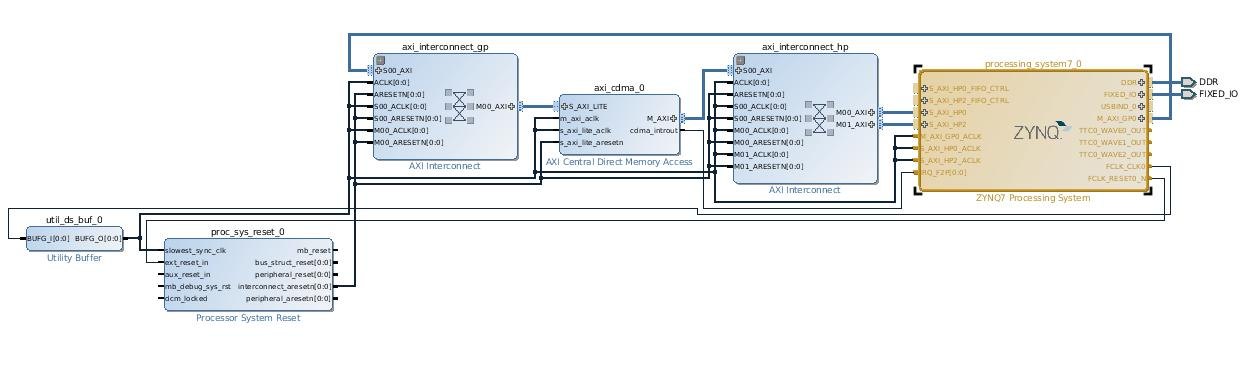
\includegraphics[scale=0.5]{figures/hardware_design.jpeg}
  \caption{Worker Control Interface - Separation of Concerns}  \label{fig:hardware_design}
  \end{center}
\end{figure}
\begin{enumerate}
\item Along the main Vivado toolbar, there is a yellow box icon with a green checkmark.  Click this icon to validate the design. When the "Validation Successful" dialogue block opens, click ok.
\item In the Sources tab/window, expand Design Sources, right-click on the top level design name, and select "Create HDL Wrapper".
\item In the dialogue box that appears, select "Let Vivado manage wrapper and auto-update" and then click ok.
\item In the Sources tab/window, right-click in the top level *.bd file, and select "Generate Output Products".  In the dialogue box that opens, click "Generate"
\end{enumerate}

\subsection{Generating Bitstream and Exporting to SDK}\label{subsec:Exporting to SDK}
\begin{enumerate}

\item In the Flow Navigator pane of Vivado, under Program and Debug, click on Generate Bitstream.
\item A pop-up window will ask whether or not to perform synthesis and implementation first.  Click "yes".  Bitstream generation can take 10 minutes or so, depending on design and computer resources.
\item Once bitstream generation is complete, a "Bitstream Generation Completed" window will appear.  Select "View Reports" to see implementation results such as device utilization, place and route details, etc.
\item To export the hardware design to SDK, click on the File menu in the upper left corner of the Vivado screen.  Navigate to Export, and click on Hardware.
\item In the Export Hardware window that appears, check the box marked "Include Bitstream".  Keep the "Export to:" field as $<$Local to Project$>$, and click "ok".  This will create a subdirectory in the vivado project folder which will contain the SDK workspace.  The subdirectory will be called $<$project name$>$.sdk.  Vivado will populate the subdirectory with initalization code and settings for the Zynq processor, DDR, clocks, PLLs and MIOs.
\item Note - If SDK does not automatically open, from the File menu, select "Launch SDK".  Keep both the Exported location and Workspace as $<$Local to Project$>$.  Click "ok".

\end{enumerate}
\section{Running an Application on Zedboard Baremetal}
% changes to cdma_app.c: had to add/change BASEADDR values as follows

% #define XPAR_PS7_DDR_0_S_AXI_HP0_BASEADDR 0x10000000
% #define XPAR_PS7_DDR_0_S_AXI_HP2_BASEADDR 0x18000000

% static u32 SourceAddr 	= XPAR_PS7_DDR_0_S_AXI_HP0_BASEADDR;
% static u32 DestAddr 	= XPAR_PS7_DDR_0_S_AXI_HP2_BASEADDR;

\section{Running an Application on Zedboard with Linux}

\subsection{Creating the CDMA Application Project in SDK}
\label{subsec:cdma_project}
Continuing from the end of section \ref{subsec:Exporting to SDK}, SDK is now open.  In the Project Explorer window, the hardware description file (*.hdf) generated from the vivado design can be seen as system.hdf under $<$vivado\_design\_name$>$\_wrapper\_hw\_platform\_0.
\label{par:SDK Open}

\begin{enumerate}
\item Select File $->$ New $->$ Application Project
\item In the dialogue box that appears, make the following selections:
\begin{itemize}
\item Project Name: linux\_cdma\_app
\item Use Default Location: yes
\item OS Platform: linux
\item Hardware Platform: $<$vivado\_design\_name$>$\_wrapper\_hw\_platform\_0 (as described in subsection \ref{subsec:new project}, item \ref{itm:project name})
\item Processor: ps7\_cortexa9\_0 (first core of the dual core A9 processor)
\item Language: C
\item Board Support Package: Create New: linux\_cdma\_app\_bsp
\end{itemize}
\item Click Next.
\item Under Avalable Templates, select Empty Application, and select "Finish"
\item Two new items will appear in the project explorer: linux\_cdma\_app and linux\_cdma\_app\_bsp.
\item Right click on the src directory under the linux\_cdma\_app, and select Import.
\item Click on General to expand, and select File System.  Click Next.
\item Browse to the unzipped UG1165 support files, and select "linux\_cdma\_app.c".  Add the file, and click Finish.  Temporarily ignore any warnings or errors.
\item Open cdma\_app.c in an editor and make the following changes:
\begin{enumerate}
\item Include a missing library
\begin{lstlisting}
#include <unistd.h>
\end{lstlisting}
\item Change CDMA\_BASE\_ADDRESS to match offset address of axi\_cdma\_0 from vivado address editor
\begin{lstlisting}
#define CDMA_BASE_ADDRESS     0x7e200000
\end{lstlisting}
\item Change DDR\_BASE\_ADDRESS to match offset address of S\_AXI\_HP0*/
\begin{lstlisting}
#define DDR_BASE_ADDRESS     0x10000000
\end{lstlisting}
\item Change DDR\_BASE\_WRITE\_ADDRESS to match offset address of S\_AXI\_HP2*/
\begin{lstlisting}
#define DDR_BASE_WRITE_ADDRESS    0x18000000
\end{lstlisting}
\item Change DDR\_MAP\_SIZE to match size of S\_AXI\_HP0 and S\_AXI\_HP2*/
\begin{lstlisting}
#define DDR_MAP_SIZE 0x5000000
\end{lstlisting}
\item Halve BUFFER\_BYTE\_SIZE
\begin{lstlisting}
#define BUFFER_BYTESIZE	131072
\end{lstlisting}

\end{enumerate}
\item The application may still fail to compile or link due to a current error in the way Vivado populates the SDK settings when it exports the design.  If this is the case, review compiler and linker scripts.  Right click on linux\_cdma\_app and go to Properties --$>$ C/C++ build --$>$ Settings --$>$ ARM Linux gcc compiler/linker.  Some of the options under the field "All options" may need to be removed.
\end{enumerate}
\subsection{Repos and Downloads}\label{subsec:repos}The following repos are required to build the linux kernal and run the design on hardware.  See table \ref{table:references} for more information.
\\

%\newline
Download these repos into the top level of the Xilinx directory on the Linux machine.  For the git repos, using the following command:

\begin{lstlisting}
	$git clone https://path.to.repo.git
\end{lstlisting}

\paragraph*{linux-xlnx.git}\label{par:linux-xlnx}https://github.com/Xilinx/linux-xlnx.git.  This repo contains the Xilinx release of the Linux kernel.  Specifically, uImage is needed for both SD card booting and JTAG booting.
\paragraph*{device-tree.git}\label{par:devicetree}https://github.com/Xilinx/device-tree-xlnx.git. This repo will be a necessary inclusion to the SDK environment in order to generate the customized device tree (devicetree.dts) for the zedboard.
\paragraph*{dtc.git}\label{par:dtc}https://git.kernel.org/pub/scm/utils/dtc/dtc.git.  For this effort, this repo will only be used to convert devictree.dts to system.dtb, a recognizable u-boot format.
\paragraph*{2015.4-zed-release}\label{par:zed}http://www.xilinx.com/Zynq+2015.4+Release - this download contains files necessary for a basic zedboard booting.  This effort uses only uramdisk.image.gz which is the zedboard-customized file system image.

\subsection{Environment}
\label{subsec:environment}
Set the environment as follows.  The provided path values assume the git repos are installed at /opt/Xilinx.
\begin{lstlisting}

	$export CROSS\_COMPILE="arm-xilinx-linux-gnueabi-"

	$export PATH="/opt/Xilinx/dtc:$PATH"

	$export PATH="/opt/Xilinx/u-boot-xlnx/tools:$PATH"
\end{lstlisting}

\subsection{Creating Zedboard Boot Files} \label{subsec:ZedboardBoot} These are the files necessary to boot and run a Linux Application on the Zedboard.  Creation and utilization of these items will be described in the sections that follow.
\begin{enumerate}
\item{\textbf{Hardware Bit File}}\label{itm:bit} - design.bit
\item{\textbf{First Stage Boot Loader}}\label{itm:fsbl} - fsbl.elf
\item{\textbf{File System Image}}\label{itm:uramdisk} - uramdisk.image.gz
\item{\textbf{Second Stage Boot Loader}}\label{itm:uboot} - u-boot.elf
\item{\textbf{Linux Kernel Image}}\label{itm:uImage} - uImage
\item{\textbf{Device Tree}}\label{itm:devicetree} - devicetree.dtb
\end{enumerate}

\subsubsection{Hardware Bit File}
The Hardware Bit File, design.bit was created in subsection \ref{subsec:Exporting to SDK}.  It was exported to the Xilinx SDK environment, and can be found at $<$Vivado Project Location$>$/$<$Vivado Project Name$>$.sdk/$<$Vivado Block Design Name$>$\_wrapper\_hw\_platform\_0/$<$Vivado Block Design Name$>$.bit
\subsubsection{First Stage Boot Loader} \label{subsec:FSBL}
The first stage bootloader is customizable for the specific platform, chip and peripherals being used.  In this effort it is created within Xilinx SDK.  It will load the Zynq chip and initialize it based upon the hardware design.

\begin{enumerate}
\item In the SDK environment, within the same workspace as begun in subsection \ref{subsec:cdma_project}, select New --$>$ Application Project.
\item  In the dialogue box that appears, make the following selections before clicking Next:
\begin{enumerate}
\item Project Name: fsbl
\item Use Default Location: yes
\item OS Platform: standalone
\item Hardware Platform: $<$vivado\_design\_name$>$\_wrapper\_hw\_plaform\_0 (as described in subsection \ref{subsec:new project}, item \ref{itm:project name})
\item Processor: ps7\_cortexa9\_0
\item Language: C
\item Board Support Package: Create New: fsbl\_bsp
\end{enumerate}
\item In the next page of the dialogue box, select Zynq FSBL Template, and click Finish.  \textbf{fsbl.elf} is created under fsbl/binaries.
\end{enumerate}
\subsubsection{File System Image}
In this effort, the rootfs (root filesystem) did not need to be rebuilt from scratch.  A standard rootfs is included in the 2015.4-zed-release archive downloaded in subsection \ref{subsec:repos}.  It is found in 2015.4\_zed\_release/zed/ and is called \textbf{uramdisk.image.gz}.
\subsubsection{Second Stage Boot Loader}
The SSBL is created using the git repo downloaded in subsection \ref{subsec:repos}.  It will load Linux onto the Zynq A9 Processor.
\begin{enumerate}
\item In a terminal window, cd to /opt/Xilinx/u-boot-xlnx.  Make sure the environment is set up as described in subsection \ref{subsec:environment}
\item Type the following and hit enter, to configure the make process for the Zedboard:
\begin{lstlisting}
$make zynq_zed_config
\end{lstlisting}
\item Type the following and hit enter, to rebuild u-boot for the Zedboard and to create the mkimage executable (can be used later to wrap u-boot headers).
\begin{lstlisting}
$make
\end{lstlisting}
*Note - compiling u-boot also creates the mkimage utility, which will be used in subsection \ref{subsec:LinuxKernel}, item \ref{itm:CreateKernel}, to wrap the linux kernel in a format that the u-boot recognizes.
\item Rename u-boot to \textbf{u-boot.elf}
\end{enumerate}
\subsubsection{Linux Kernel Image} \label{subsec:LinuxKernel}
\begin{enumerate}
\item cd to /opt/Xilinx/linux-xlnx and
\item type the following to configure the kernel based on the contents of linux-xlnx/arch/arm/configs/xilinx\_zynq\_defconfig:
\begin{lstlisting}
make ARCH=arm xilinx_zynq_defconfig
\end{lstlisting}
\item type the following for an interactive menu allowing additional kernel configuration:
\begin{lstlisting}
make ARCH=arm menuconfig
\end{lstlisting}
\item type the following to create the kernel: \label{itm:CreateKernel}
\begin{lstlisting}
make ARCH=arm UIMAGE_LOADADDR=0x8000 uImage
\end{lstlisting}
uImage will be created at /opt/Xilinx/linux-xlnx/arch/arm/boot.\\
*Note - If uImage does not appear at this location, but Image and zImage is created, then the mkimage utility (in the u-boot-xlnx repo) has not been added to the build environment path as described in subsection \ref{subsec:environment}.
\end{enumerate}
\subsubsection{Device Tree}
The Device Tree identifies all of the hardware devices for the Linux kernel.
\begin{enumerate}
\item  cd to /opt/Xilinx/dtc and type
\begin{lstlisting}
$make
\end{lstlisting}
\item Ensure the terminal window PATH points to dtc, as described in section \ref{subsec:environment}.
\item In the SDK environment, continuing in the workspace from subsection \ref{subsec:FSBL}, select from the main menu, Xilinx Tools --$>$ Repositories.
\item In the dialogue box that appears, click "New" in the Local Repositories area.
\item Browse to the directory /opt/Xilinx/device-tree-xlnx, and click "ok".\label{itm:repo}
\item From the main menu, select File --$>$ New --$>$ Board Support Package.
\item In the dialogue box that appears, ensure the following options are selected.
\begin{enumerate}
\item Project name: devie\_tree\_bsp
\item Use default loaction: checked
\item Target Hardware Platform: $<$Vivado\_design\_name$>$\_wrapper\_hw\_platform\_0
\item Target CPU: ps7\_cortexa9\_0
\item Board Support Package OS: device\_tree
\\ *Note "device\_tree" will only appear in the Board Support Package OS type list if the device-tree-xlnx repository was correctly added as described in list item \ref{itm:repo} above.
\end{enumerate}
\item Click "Finish".
\item System.mss will be created, and can be viewed in the Project Explorer pane under device\_tree\_bsp\_0.  The file can be modified by double-clicking it, and then clicking the button "Modify this BSP's Settings"
\item In the terminal window, cd to the path of system.mss, and type
\begin{lstlisting}
dtc -I dts -O dtb -o devicetree.dtb system.dts
\end{lstlisting}
This converts the name and file type of system.dts to devicetree.dtb, which is necessary for u-boot to recognize the device tree upon loading.
\end{enumerate}

\subsection{Booting Zedboard With an SD Card and Running the Linux Application}
\subsubsection{Board Settings}
\begin{enumerate}
\item The MIO bank on the Zedboard must have the following values to enable booting from SD card:
\begin{itemize}
\item MIO6 GND
\item MIO5 3.3V
\item MIO4 3.3V
\item MIO3 GND
\item MIO2 GND
\end{itemize}
\item Ensure the Platform USB Cable is connected between the host machine and the Zedboard JTAG port.
\item Ensure the UART cable is connected from the host machine to the Zedboard UART port.
\item Ensure the UART port is enabled on the Zedboard by shunting the JP3 pins.
\item Ensure the power cable is plugged into the board.
\item Ensure the ethernet cable is plugged into the board.
\end{enumerate}
\subsubsection{Creating BOOT.bin}
The Zynq Boot Image is a compilation of elements already created in previous sections.  In this effort, SDK is used to put the necessary components into BOOT.bin
\begin{enumerate}
\item In the SDK environment used in subsection \ref{subsec:ZedboardBoot}, from the main menu, select Xilinx Tools --$>$ Create Zynq Boot Image.
\item In the dialogue box that appears, select the following parameters:
\begin{enumerate}
\item Output File Path: path/to/$<$Vivado\_design\_name$>$\_wrapper\_hw\_platform\_0
\item Use Authentication: unchecked
\item Use Encryption: unchecked
\item Boot image partitions: Click "Add" to add the files below. *Note - order is important!
\begin{enumerate}
\item fsbl.elf - located in workspace under fsbl/binaries
\item design.bit - located in workspace under/$<$Vivado Block Design Name$>$\_wrapper\_hw\_platform\_0/$<$Vivado Block Design Name$>$.bit
\item uboot.elf - located at /opt/Xilinx/u-boot-xlnx/uboot.elf
\end{enumerate}
\end{enumerate}
\item click "Create Image".
\item BOOT.bin will be created in workspace under fsbl/bootimage
\end{enumerate}
\subsubsection{Loading and Booting from the SD Card}\label{subsubsec:SD}
\begin{enumerate}
\item Load the following files onto an SD Card to boot and run a linux application:
\begin{itemize}
\item \textbf{Zynq Boot Image} - BOOT.bin
\item \textbf{Device Tree} - devicetree.dtb
\item \textbf{Linux Kernel} - uImage
\item \textbf{File System Image} - uramdisk.image.gz
\end{itemize}
\item Remove the SD card from the computer and (with Zedboard off) insert into the flash port on the underside of the Zedboard.
\item Flip the Zedboard switch into the "on" position.
\item Open a serial terminal window emulator.  In this effort minicom is used.  To open a minicom window and communicate with the Zedboard via serial port, type: \label{itm:minicom}
\begin{lstlisting}
minicom -b 115200 -D /dev/ttyACM0
\end{lstlisting}
If the initial boot is finished when the minicom screen links to the serial port, the screen will display:
\begin{lstlisting}
Zynq>
\end{lstlisting}
\item In the minicom window, type "boot" and hit enter.
\item If Linux boots successfully, boot information will scroll by, ending with the following:
\begin{lstlisting}
Starting syslogd/klogd: done
Starting tcf-agent: OK
zedboard-zynq7 login:
\end{lstlisting}
\item Type "root" for the Zedboard username/password and hit enter.
\item Type "ifconfig" to display the IP address acquired by the Zedboard.
\end{enumerate}
\subsubsection{Running the CDMA Application}
The CDMA Application modified in subsection \ref{subsec:cdma_project} will now be tranferred to and run on the Zedboard.
\begin{enumerate}
\item In a terminal window, cd to linux\_cdma\_app/Debug/
\item Type the following:
\begin{lstlisting}
sudo scp ./linux_cdma_app.elf <IP address of Zedboard>:/home/root
\end{lstlisting}
\item In the Project Explorer pane of Xilinx SDK, right click on cdma\_app and select Run As --$>$ Launch on Hardware (GDB)
\item In the minicom window, type:
\begin{lstlisting}
./linux_cdma_app.elf
\end{lstlisting}
Successful execution will yield the following display in the minicom window:
\begin{lstlisting}
Entering Main
/dev/mem opened.
Memory mapped at address 0xb1fc4000.
DATA Transfer is Successfull
\end{lstlisting}
\end{enumerate}

\subsection{Booting Zedboard Over JTAG and Running the Linux Application}
Booting over JTAG allows one useful benefit: The ability to utilize Xilinx SDK's GDB Debug environment while executing an application on the Zedboard.

\subsubsection{Board Settings}
\begin{enumerate}
\item The MIO bank on the Zedboard must have the following values to enable booting over JTAG:
\begin{itemize}
\item MIO6 GND
\item MIO5 GND
\item MIO4 GND
\item MIO3 GND
\item MIO2 GND
\end{itemize}
\item Ensure the Platform USB Cable is connected between the host machine and the Zedboard JTAG port.
\item Ensure the UART cable is connected from the host machine to the Zedboard UART port.
\item Ensure the UART port is enabled on the Zedboard by shunting the JP3 pins.
\item Ensure the power cable is plugged into the board.
\item Ensure the ethernet cable is plugged into the board.
\end{enumerate}
\subsubsection{Loading and Booting over JTAG}
In the following instructions, fsbl.elf is not used, as it has not been shown to work in this effort.  Instead, a tcl script released by Xilinx is used.
\begin{enumerate}
%\item Open a minicom window as described in subsubsection \ref{subsubsec:SD}, item \ref{itm:minicom}
\item Withing the Xilinx SDK workspace, use the SDK Terminal for serial input and output.  If one is not open in the C/C++ perspective, then in the main menu click on Window --$>$ Show View --$>$ Other --$>$ Xilinx --$>$ SDK Terminal, and then click "OK".
\item In the SDK Terminal window, click on the green "+" sign to open a new serial port.  Set the baudrate to 115200.  In this effort the port was located at /dev/ttyACM0.  Click OK.
\item Also within the Xilinx SDK workspace, locate the Xilinx XMD Console.  If it is not open, on the main menu, select Xilinx Tools --$>$ XMD Console.
\item In the XMD console, type and enter each of the following commands:
\\ *Note - Alternatively, these commands may be put in a file and run by simply typing "source $<$filename$>$"
\begin{enumerate}
\item cd $<$path/to/$<$Vivado Block Design Name$>$\_wrapper\_hw\_platform\_0/$>$
\item connect arm hw
\item fpga -f $<$Vivado Block Design Name$>$.bit
\item source stub.tcl
\item target 64
\item source ps7\_init.tcl
\item ps7\_init
\item ps7\_post\_config
\item dow -data /opt/Xilinx/linux-xlnx/arch/arm/boot uImage 0x03000000
\item dow -data device\_tree\_bsp\_0/devicetree.dtb 0x02a00000
\item dow -data /opt/Xilinx/2015.4\_zed\_release/zed/uramdisk.image.gz 0x02000000
\item dow /opt/Xilinx/linux-xlnx/u-boot.elf
\item con
\end{enumerate}
\item In the SDK Terminal window, some u-boot output will appear.  When "Hit any key to stop autoboot" appears, hit any key and the "zynq-uboot" prompt will appear.
\item In the SDK Terminal window, type:
\begin{lstlisting}
bootm 0x03000000 0x02000000 0x02a00000
\end{lstlisting}
\item After Linux boots, the prompt will be zedboard-zynq7.  Enter the username/password of "root".
\end{enumerate}
\subsubsection{Running the CDMA Application}
\begin{enumerate}
\item In Xilinx SDK, right click on linux\_cdma\_app and select Debug as --$>$ Debug Configurations...

\item In the dialogue box that appears, in the left menu pane, select "Remote ARM Linux Application".  \\
*Note - If that listing is not available, click the pane menu pull-down icon \, "\raisebox{-5pt}{\bf\large{\v{}}}" and uncheck "Filter Configuration Types".
\item Once "Remote ARM Linux Application is selected", click the "New" icon to create a new ARM Linux Application configuration>
\item In the dialogue box that appears, next to Connection, click "New...".  A "New Connection dialogue box will appear.  Select the following options and then click "Finish":
\begin{enumerate}
\item System type: Linux (click "Next)
\item Parent profile: $<$default$>$
\item Host name: $<$IP address of Zedboard$>$
\item Connection name: $<$IP address of Zedboard$>$
\item Description: $<$IP address of Zedboard$>$
\end{enumerate}
\item In the Debug Configurations dialogue box, select the following options:
\begin{enumerate}
\item Connection: $<$IP address of Zedboard$>$
\item Project: linux\_cdma\_app
\item Select configuration using 'C/C++ Application': checked
\item C/C++ Application: Debug/linux\_cdma\_app.elf
\item Remote Absolute File Path for C/C++ Application:/home/root/linux\_cdma\_app.elf //
*Note - Make sure the elf executable is listed in the path for it to be recognized!
\item Skip download to target path: unchecked
\item Click "Apply"
\end{enumerate}

\item In the dialogue box that appears, select "Xilinx C/C++ application(GDB).
\item Click on the "New" icon and enter the following parameters:
\begin{enumerate}
\item Debug Type: Standalone Application Debug
\item Connection: zed\_ssh %give directions on how to create this!
\item Device: Auto Detect
\item Hardware platform: $<$Vivado Block Design Name$>$\_wrapper\_hw\_platform\_0
\item Processor: ps7\_cortexa9\_0
\item Bitstream file: $<$Vivado Block Design Name$>$.bit
\item Initialization file: ps7\_init.tcl
\item Reset selection: No reset
\item Run ps7\_init: unchecked
\item Run ps7\_post\_config: unchecked
\item Enable Cross-Triggering: unchecked
\end{enumerate}
\item Click "Apply"
\item Return to the Remote ARM Linux Application - linux\_cdma\_app Debug configuration pane.  Click "Close".
\item In the SDK Main Menu, click Window --$>$ Perspective --$>$ Open Perspective --$>$ Other --$>$ Remote Systems Explorer. \label{itm:RemoteSystemsExplorer}
\item Within the Remote System Explorer perspective, click Window --$>$ Show View --$>$ Other --$>$ Remote Systems --$>$ Remote Monitor.
\item Within the Remote Monitor pane, right click on SSH Terminals and select Connect...
\item In the dialogue box that appears, enter the User ID and Password (root) and click "OK".
\item If a warning appears about inserting a new key into .ssh/known\_hosts, click "Yes".
\item The SSH Terminals should now appear as Connected in the Remote Monitor Pane.\label{itm:SshConnected}
\\ *Note - In this effort, connecting via SSH automatically by clicking on Debug In the Debug Configurations dialogue box did not work.  Thus the manual connection described in steps \ref{itm:RemoteSystemsExplorer} through \ref{itm:SshConnected}.
\item Return to the C/C++ perspective.
\item Right click on linux\_cdma\_app and select Debug As --$>$ Debug Configurations.
\item Navigate to Remote ARM Linux Application --$>$ linux\_cdma\_app Debug.
\item Click on "Debug" in the lower right corner of the dialogue box.
\item The Debug perspective will automatically open.  If linux\_cdma\_app.c is not already open, from the main menu select File --$>$ Open File, browse to the file and click "OK". Set and step through breakpoints using the menu icons.
\item Click on the Console tab to view program output.
\item A successful program run will end with the Console messages below:
\begin{lstlisting}
DATA Transfer is Successful

Child exited with status 0
GDBserver exiting
root@zedboard-zynq7:~# exit
logout
\end{lstlisting}
\end{enumerate}
\section{Appendix}
\subsection{Troubleshooting}

\end{document}
